

\subsection{Требования к времени когеренции пучка}
Время когеренции спина (spin coherence time; SCT) для метода
замороженного спина, выполненного в накопительном кольце с идеально
установленными элементами определяется минимальным детектируемым углом
отклонения вектора поляризации пучка из горизонтальной плоскости
только засчёт ЭДМ. Для уровня чувствительности $10^{-29}~e\cdot cm$
это примерно $5\cdot10^{-6}$.~\cite{BNL:Deuteron2008}

В соответствии с уравнением Т-БМТ,
\[
\W_{EDM,x} = \eta\frac{qE_x}{2mc},
\]
где $\eta$ есть коэффициент пропорциональности между ЭДМ и спином,
равный $10^{-15}$ для дейтрона, для данного уровня чувствительности.~\cite[стр.~206]{Eremey:Thesis}

Для дейтронного BNL FS кольца, $E_x = 12$
МВ/м,~\cite[стр.~19]{BNL:Deuteron2008} так что $\W_{EDM,x}\approx
10^{-9}$ рад/сек. Таким образом получаем, что для того, чтобы достичь
детектируемый уровень отклонения вектора поляризации на 1 мкрад требуется SCT порядка 1000 секунд.~\cite[стр.~207]{Eremey:Thesis}
\subsection{Происхождение декогеренции}
Декогеренция спина в пучке вызвана разницей угловых скоростей
прецессии спинов частиц, которая, в свою очередь, вызвана разницей
длин орбит и импульсов частиц. Это можно видеть исходя из следующих
соображений.

Когда частица со спином входит в область магнитного поля, её спин-вектор
начинает поворачиваться вокруг вектора магнитного поля с угловой
скоростью определяемой уравнением Т-БМТ~\eqref{eq:TBMT_MDM}:
\begin{equation*}
	\vec\W_{MDM} = \frac qm G\vec B.
\end{equation*}
На выходе из области, вектор спина повёрнут на угол
\begin{equation*}
	\theta = \Delta t\cdot\W_{MDM} = \frac Lv \cdot \frac qm GB\cdot \frac{\gamma_0}{\gamma_0} = \frac{L\gamma_0 GB}{B\rho} = \frac L\rho\gamma_0\cdot G,
\end{equation*}
где $L$ есть длина пути внутри области с магнитным полем, и $B\rho =
p/q$ магнитная жёсткость.

В простой модели рассмотренной выше, влияние орбитальной динамики на
спиновую динамику выражено через $\gamma_0 L/\rho$ (эффективный
Лоренц-фактор). В случае референсной частицы, $\gamma_0L/\rho =
\gamma_0\alpha$, $\alpha$ угол поворота вектора импульса, в то время
как для частицы участвующей в бетатронном движении, эффективный
Лоренц-фактор больше. В следующих разделах мы выразим связь между
спиновой и орбитальной динамиками частицы в накопительном кольце в
более общих терминах.

\paragraph{Сдвиг равновесного значения импульса частицы.}
Продольная динамика заряженной частицы на референсной орбите в
накопительном кольце описывается системой уравнений
\begin{equation*}
	\begin{cases}
		\ddt{\varphi} &= -\w_{RF}\eta\delta, \\
		\ddt{\delta} &= \frac{q V_{RF}\w_{RF}}{2\pi h\beta^2E}\sin\varphi.
	\end{cases}
\end{equation*}
В уравнениях выше: $\varphi$ отклонение фазы частицы от референсной
$\varphi_0 = 0$; $\delta = \frac{\Delta p}{p_0}$ относительное
отклонение импульса от $p_0$ референсной частицы; $V_{RF}$, $\w_{RF}$
амплитуда и частоты колебаний ВЧ поля; $\eta = \alpha_0 - \gamma^{-2}$
слип-фактор, где $\alpha_0$ --- коэффициент сжатия орбиты, определяемый
через $\sfrac{\Delta L}{L} = \alpha_0\delta$, $L$ длина орбиты; $h$
гармоническое число; $E$ полная энергия ускоряемой частицы. $\w_{RF} =
2\pi h f_{rev}$, где $f_{rev}=T_{rev}^{-1}$ --- частота оборота пучка.

Решения этой системы формируют семейство эллипсов в плоскости
$(\varphi, \delta)$, центрированных на $(0,0)$. Однако, если
рассмотреть частицу, участвующую в бетатронных колебаниях, и
использовать разложение Тейлора более высокого порядка для
коэффициента сжатия орбиты $\alpha = \alpha_0 + \alpha_1\delta$,
первое уравнение системы превратится в:~\cite[стр.~2579]{Senichev:IPAC13}
\[
\ddt{\varphi} = -\w_{RF} \bkt*{\bkt{\frac{\Delta L}{L}}_\beta + \bkt{\alpha_0 + \gamma^{-2}}\delta + \bkt{\alpha_1 - \alpha_0\gamma^{-2} + \gamma^{-4}}\delta^2},
\]
где $\bkt{\frac{\Delta L}{L}}_\beta =
\frac{\pi}{2L}\bkt*{\varepsilon_xQ_x + \varepsilon_yQ_y},$ есть
удлинение орбиты, связанное с бетатронным движением; $\varepsilon_x$ и
$\varepsilon_y$ --- горизонтальный и вертикальный эмиттансы пучка, и
$Q_x$ и $Q_y$ горизонтальный и вертикальный тюны.~\cite[стр.~2580]{Senichev:IPAC13}

Решения модифицированной системы более не центрированы на одной и той
же точке. Удлинение орбиты и отклонение импульса вызывают сдвиг
равновесного значения импульса частицы~\cite[стр.~2581]{Senichev:IPAC13}
\begin{equation}\label{eq:EquLevMom_shift}
\Delta\delta_{eq} = \frac{\gamma_0^2}{\gamma_0^2\alpha_0 - 1}\bkt*{\frac{\delta_m^2}{2}\bkt{\alpha_1 - \alpha_0\gamma^{-2} + \gamma_0^{-4}} + \bkt{\frac{\Delta L}{L}}_\beta},
\end{equation}
где $\delta_m$ --- амплитуда синхротронных колебаний.

\paragraph{Понятие эффективного Лоренц-фактора.}
Равновесное значение энергии, связанное со сдвигом импульса~\eqref{eq:EquLevMom_shift}, и называемое \emph{эффективным Лоренц-фактором}, есть~\cite{Senichev:FDM}
\begin{equation}\label{eq:EffectiveGamma}
\gamma_{eff} = \gamma_0 + \beta_0^2\gamma_0\cdot\Delta\delta_{eq},
\end{equation}
где $\gamma_0$, $\beta_0$ --- Лоренц-фактор референсной частицы и
нормализованное значение
скорости. Уравнения~\eqref{eq:EquLevMom_shift}
и~\eqref{eq:EffectiveGamma} определяют связь между спиновой и
орбитальной динамиками частицы.

Из уравнения для спин-тюна частицы в магнитном поле $\nu_s = \gamma_{eff}\cdot G$ следует, что спин-тюны двух частиц с одинаковыми эффективными Лоренц-факторами равны, независимо от их траекторий в ускорителе. Этот принцип используется при использовании секступольных полей для подавления спиновой декогеренции, а также при смене полярности ведущего магнитного поля кольца.

\subsection{Подавление декогеренции с помощью секступольных полей}\label{sec:sextupole_spin_dec_solution}
Чтобы минимизировать декогеренцию спина, связанную с бетатронным
движением и отклонением импульса, могут быть использованы
секступольные (или октупольные) поля~\cite[стр.~212]{Eremey:Thesis}

Секступоль силы
\[
S_{sext} = \frac{1}{B\rho} \pddx{B_y}[x][2],
\]
где $B\rho$ магнитная жёсткость, влияет на коэффициент сжатия орбиты
первого порядка как~\cite[стр.~2581]{Senichev:IPAC13}
\begin{align}
	\Delta \alpha_{1,sext} &= -\frac{S_{sext}D_0^3}{L}, \label{eq:Sext_compaction_effect}
	\intertext{и одновременно на длину орбиты как}
	\bkt{\frac{\Delta L}{L}}_{sext} &= \mp \frac{S_{sext}D_0\beta_{x,y}\varepsilon_{x,y}}{L}, \label{eq:Sext_OL_effect}
\end{align}
где $D(s,\delta) = D_0(s) + D_1(s)\delta$ обозначает функцию дисперсии.

В следующих разделах мы будем называть декогеренцию, связанную си
горизонтальными/вертикальными бетатронными, и синхротронными
колебаниями соответственно X-/Y-, и D-декогеренцией. 

Из уравнений~\labelcref{eq:Sext_compaction_effect,eq:Sext_OL_effect} можно
видеть, что для подавления декогеренции необходимы три семейства
секступолей, помещённых в максимумы функций: $\beta_x$, $\beta_y$ для подавления
X-,Y-декогеренции, и $D_0$ для D-декогеренции.

\subsection{Симуляция эксперимента по подавлению декогеренции}
При проведении нижеследующих тестов симулировалась инжекция
плоского, гауссовского пучка в структуру с замороженным
спином. E+B спин-ротаторы в структуре были установлены со случайно распределённым углом наклона вокруг оптической оси, взятым из распределения $N(0, 5\cdot10^{-4})$ (углы в радианах).

Инжектируемые пучки состояли из 30 частиц, распределённых в
плоскости $y-z$ как $y\sim N(y_0, 0.1)$ [мм]; $x,d =
0$. Оффсет $y_0$ варьировался в диапазоне $[-1, +1]$ мм. Начальное
направление спин-векторов всех частиц --- продольное: $\vec S(t=0) = (0,0,1)$.

Также в структуре варьировалось значение градиента GSY секступоля,
модулирующего декогеренцию в вертикальной плоскости. GSY менялся в
диапазоне $[GSY0 - 5\cdot10^{-3}, GSY0 + 5\cdot10^{-3}]$, где
$GSY0=-2.5\cdot 10^{-3}$ --- оптимальное значение градиента для идеальной структуры.

На каждое значение градиента приходится 10 инжекций.

Для того, чтобы обеспечить устойчивость процедуры TSS COSY Infinity~\cite{COSYINF:BeamPhysMan}, пучок инжектировался на энергии 270 МэВ (строгий FS находится на энергии 270.0092 МэВ), а матрицы перехода орбитального и спинового движений строились до третьего порядка разложения ряда Тейлора. 

Далее ансамбль начальных значений, представляющий пучок, трекается
через структуру на протяжении $1.2\cdot10^6$ оборотов, что
примерно эквивалентно 1.2 секундам. Каждые 800 оборотов производится
запись необходимых для анализа данных.

Собираемые данные: 
\begin{enumerate*}[\itshape a\upshape)]
	\item результаты вычислений процедуры TSS: спин-тюн $\nu_s$ и компоненты вектора оси инвариантного спина $\bar n$, а также
	\item компоненты спина $(S_X, S_Y, S_Z)$, и фазового пространства $(X,A,Y,B,T,D)$.
\end{enumerate*}

Из данных по компонентам спина вычисляется поляризация банча по
формуле
\begin{equation}\label{eq:polarization_formula}
\vec P = \frac{\sum_i\vec s_i}{|\sum_i\vec s_i|}.
\end{equation}

Поляризация фиритуется функцией $f(t; a,f,\phi) = a\cdot \sin(2\pi\cdot
f\cdot t + \phi)$, оцениваются все три параметра $(\hat a, \hat f,
\hat\phi)$. 

\subsection{Анализ эффекта подавления декогеренции спина в вертикальной плоскости при помощи секступолей}
На Рисунке~\ref{fig:ny_vs_y0_GSY} представлена зависимость вертикальной компоненты оси прецессии частицы от её смещения от референсной орбиты в вертикальном направлении. Из Рисунка~\ref{fig:ny_vs_y0_GSY_full} видно, что существует некоторое значение градиента секступоля, при котором $\bar n_y(y) = \bar n_y(0)$ для всех частиц в диапазоне $\pm 1$ мм от референсной орбиты. Обратим внимание на то, что на Рисунке~\ref{fig:ny_vs_y0_GSY_zoom} наблюдается чётность функции $\Delta\bar n_y \equiv \bar n_y(y) - \bar n_y(0)$.

\begin{figure}[h!]
	\centering
	\hfill
	\subbottom[Полный диапазон.\label{fig:ny_vs_y0_GSY_full}]{%
		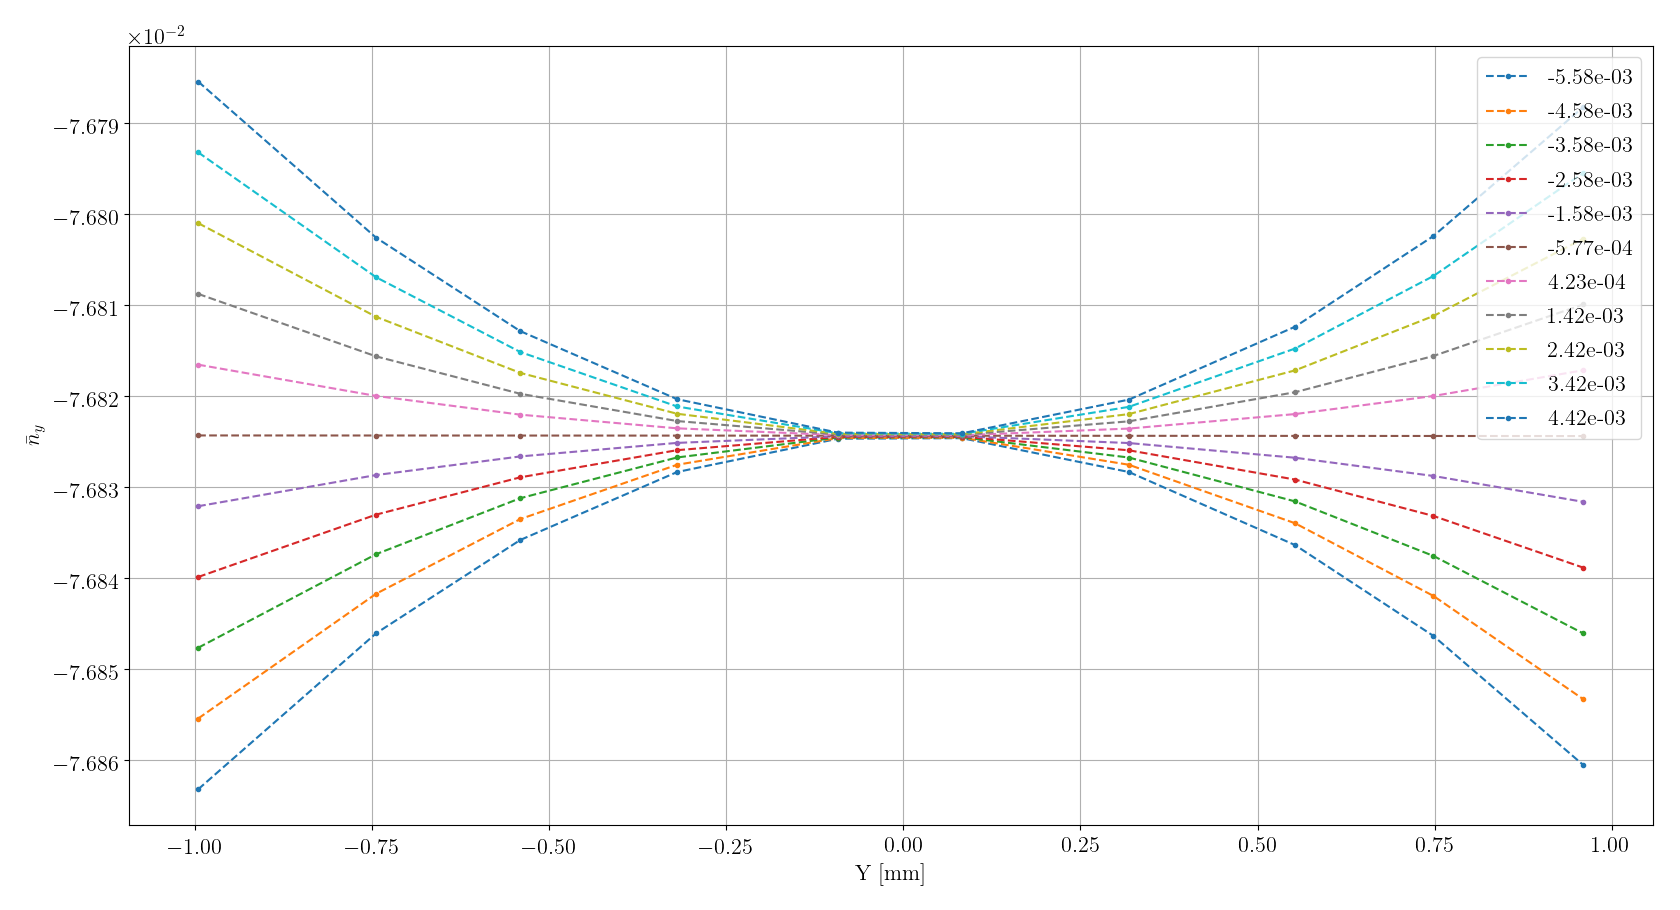
\includegraphics[width=\linewidth]{images/decoh_sim/ny_vs_offset}}
	\hfill
	\subbottom[Деталировка кривой при оптимальном значении GSY.\label{fig:ny_vs_y0_GSY_zoom}]{%
		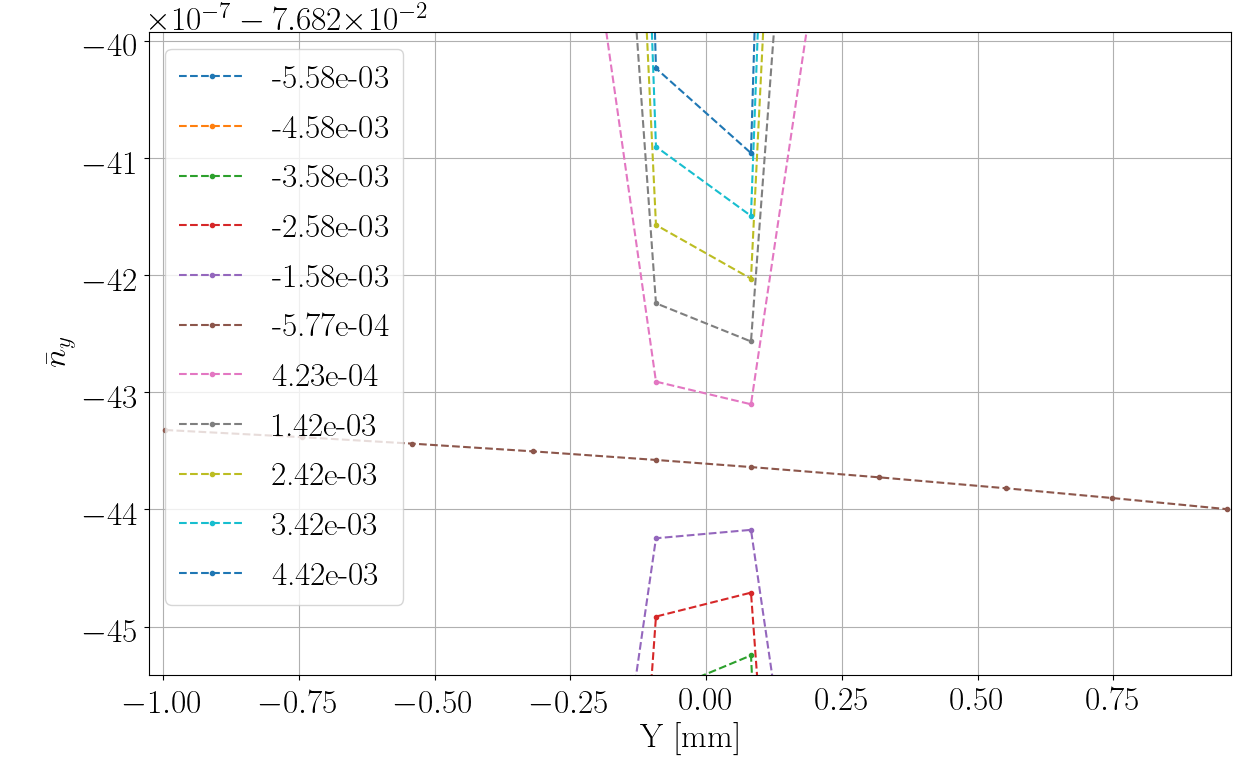
\includegraphics[width=\linewidth]{images/decoh_sim/ny_vs_offset_zoom}}
	\hfill
	\legend{Цветом обозначены данные для различных значений градиента GSY Y-секступоля.}
	\caption{Вертикальная компонента $\bar n_y$ оси прецессии спина в зависимости от смещения частицы от референсной орбиты.\label{fig:ny_vs_y0_GSY}}
\end{figure}

На Рисунке~\ref{fig:spin_tune_vs_y0_GSY} представлена зависимость спин-тюна от вертикального смещения частицы от референсной орбиты. Видно, что $\Delta\nu_s \equiv \nu_s(y) - \nu_s(0)$ --- нечётная функция.
\begin{figure}[h!]
	\centering
	\hfill
	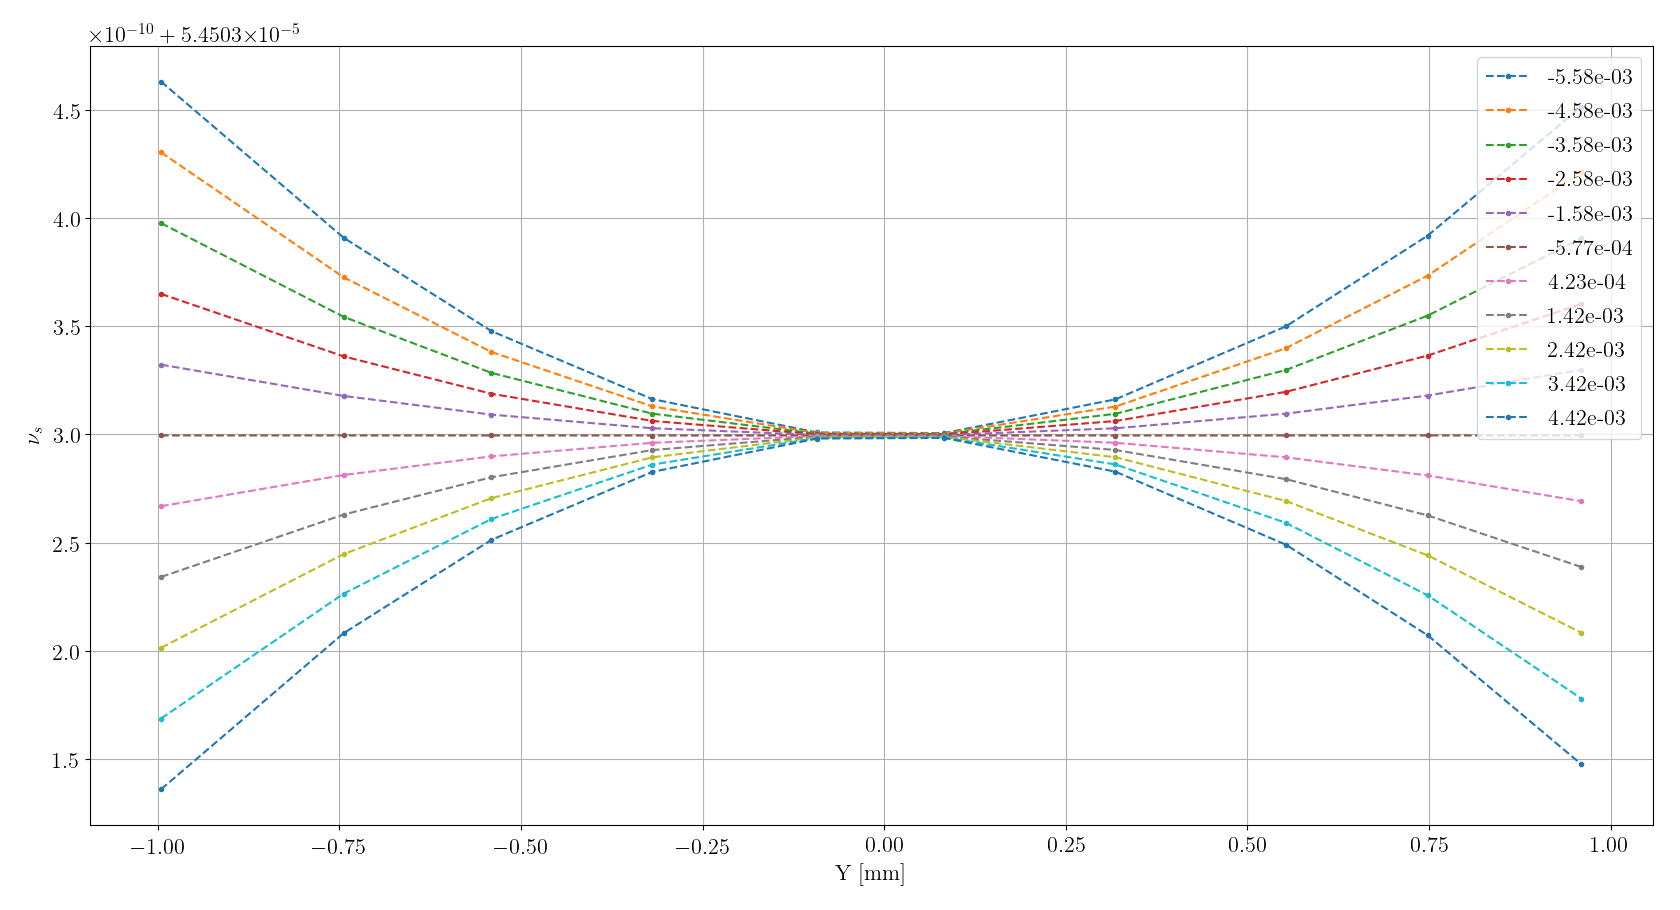
\includegraphics[width=\linewidth]{images/decoh_sim/spin_tune_vs_offset}
	\hfill
	\legend{Цветом обозначены данные для различных значений градиента GSY Y-секступоля.}
	\caption{Спин-тюн $\nu_s$ в зависимости от смещения частицы от референсной орбиты.\label{fig:spin_tune_vs_y0_GSY}}
\end{figure}

На Рисунке~\ref{fig:freq_y_vs_y0} представлена зависимость оценки частоты колебаний вертикальной компоненты поляризации банча, вычисленной по формуле~\eqref{eq:polarization_formula}, в зависимости от его начального смещения, для трёх значений градиента GSY. Из Рисунка~\ref{fig:freq_y_vs_y0_zoom} видно, что функция $\Delta\hat f \equiv \hat f(y) - \hat f(0)$--- нечётная, как и $\Delta\nu_s$. Это служит ещё одним косвенным свидетельством того, что вариация спин-тюнов частиц играет более значимую роль в оценке частоты прецессии спина,
чем модельное несоответствие, вызванное колебанием оси стабильного спина.
\begin{figure}[!h]
	\centering
	\hfill
	\subbottom[Полный диапазон.\label{fig:freq_y_vs_y0_full}]{%
		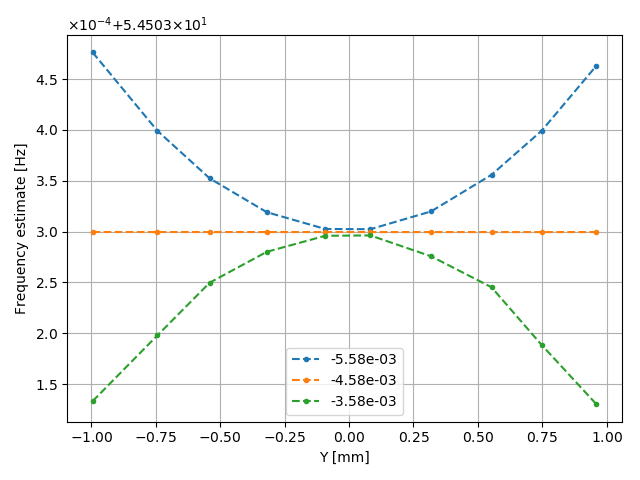
\includegraphics[width=\linewidth]{images/decoh_sim/FreqY_vs_offset}}
	\hfill
	\subbottom[Деталировка кривой при оптимальном значении градиента GSY Y-секступоля.\label{fig:freq_y_vs_y0_zoom}]{%
		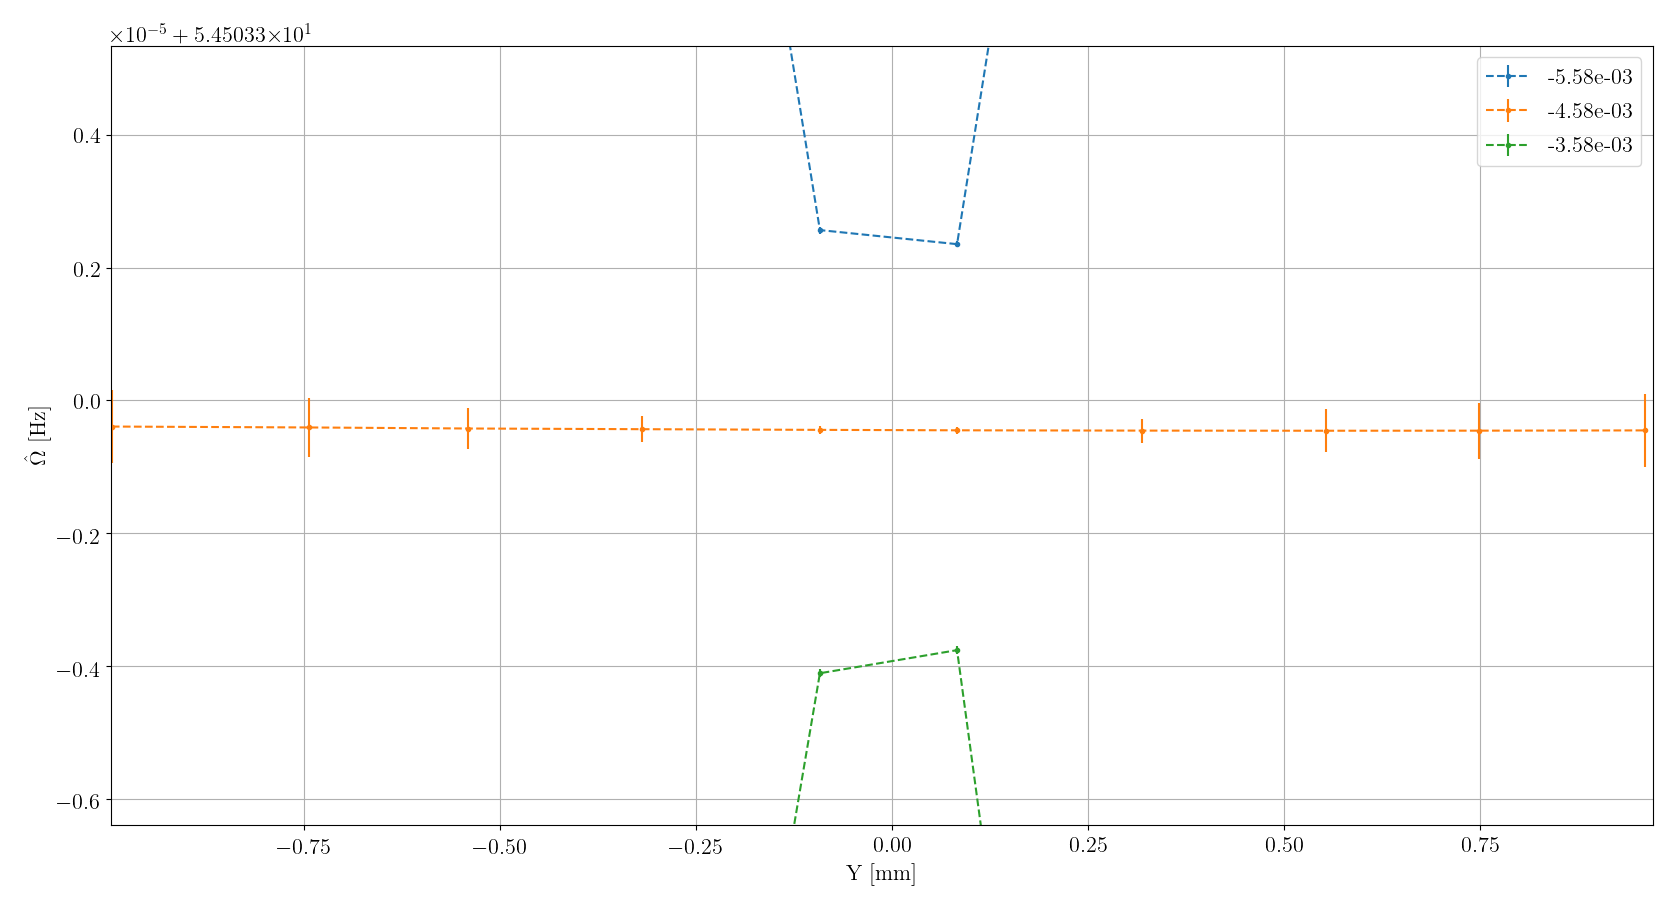
\includegraphics[width=\linewidth]{images/decoh_sim/FreqY_vs_offset_zoom}}
	\hfill
	\legend{Цветом обозначены кривые при различных значениях градиента GSY Y-секступоля.}
	\caption{Оценка частоты колебаний вертикальной компоненты поляризации в зависимости от начального смещения пучка от референсной орбиты.\label{fig:freq_y_vs_y0}}
\end{figure}

На Рисунке~\ref{fig:yb_traj} изображены траектории частиц в плоскости $(Y,B)$ фазового пространства, плоученные в результате трекинга через неидеальный ускоритель.
\begin{figure}[h!]
	\centering
	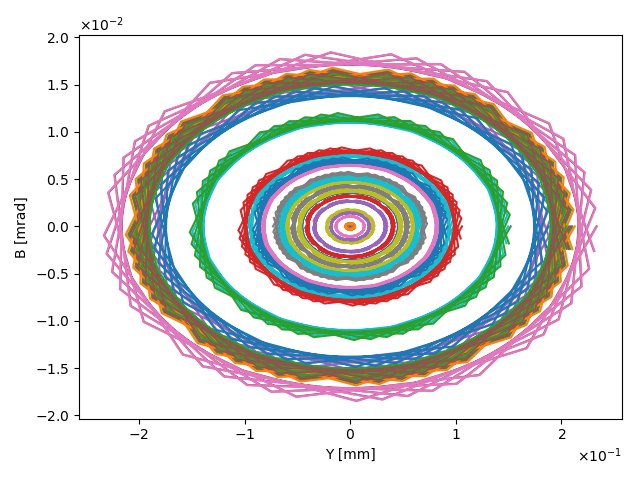
\includegraphics[width=\linewidth]{images/decoh_sim/YB-PHASE_SPACE_IMPERFECT_UNOPT}
	\caption{Траектории частиц в плоскости $(Y,B)$ фазового пространства.\label{fig:yb_traj}} 
\end{figure}

На Рисунках~\ref{fig:spin_tune_on_traj} и~\ref{fig:ny_on_traj} изображены, соответственно, спин-тюн и вертикальная компонента оси прецессии спина, вычисленные на траекториях частиц из Рисунка~\ref{fig:yb_traj}, в случае с выключенными и включенными секступолями, подавляющими декогеренцию в вертикальной плоскости. 
\begin{figure}[!h]
	\centering
	\subbottom[С выключенными секступолями.]{%
		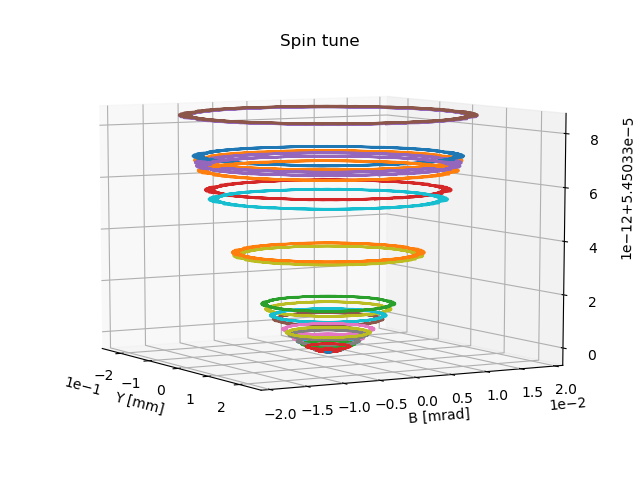
\includegraphics[width=\linewidth]{images/decoh_sim/ST_VS_YB_IMPERFECT_UNOPT}}
	\hfill
	\subbottom[С включенными секступолями.]{%
		\includegraphics[width=\linewidth]{images/decoh_sim/St_VS_YB_IMPERFECT_OPTIM}}
	\hfill
	\caption{Спин-тюны и направления оси стабильного спина частиц в неидеальной FS-труктуре.\label{fig:spin_tune_on_traj}}
\end{figure}

\begin{figure}[!h]
	\centering
	\subbottom[С выключенными секступолями.]{%
		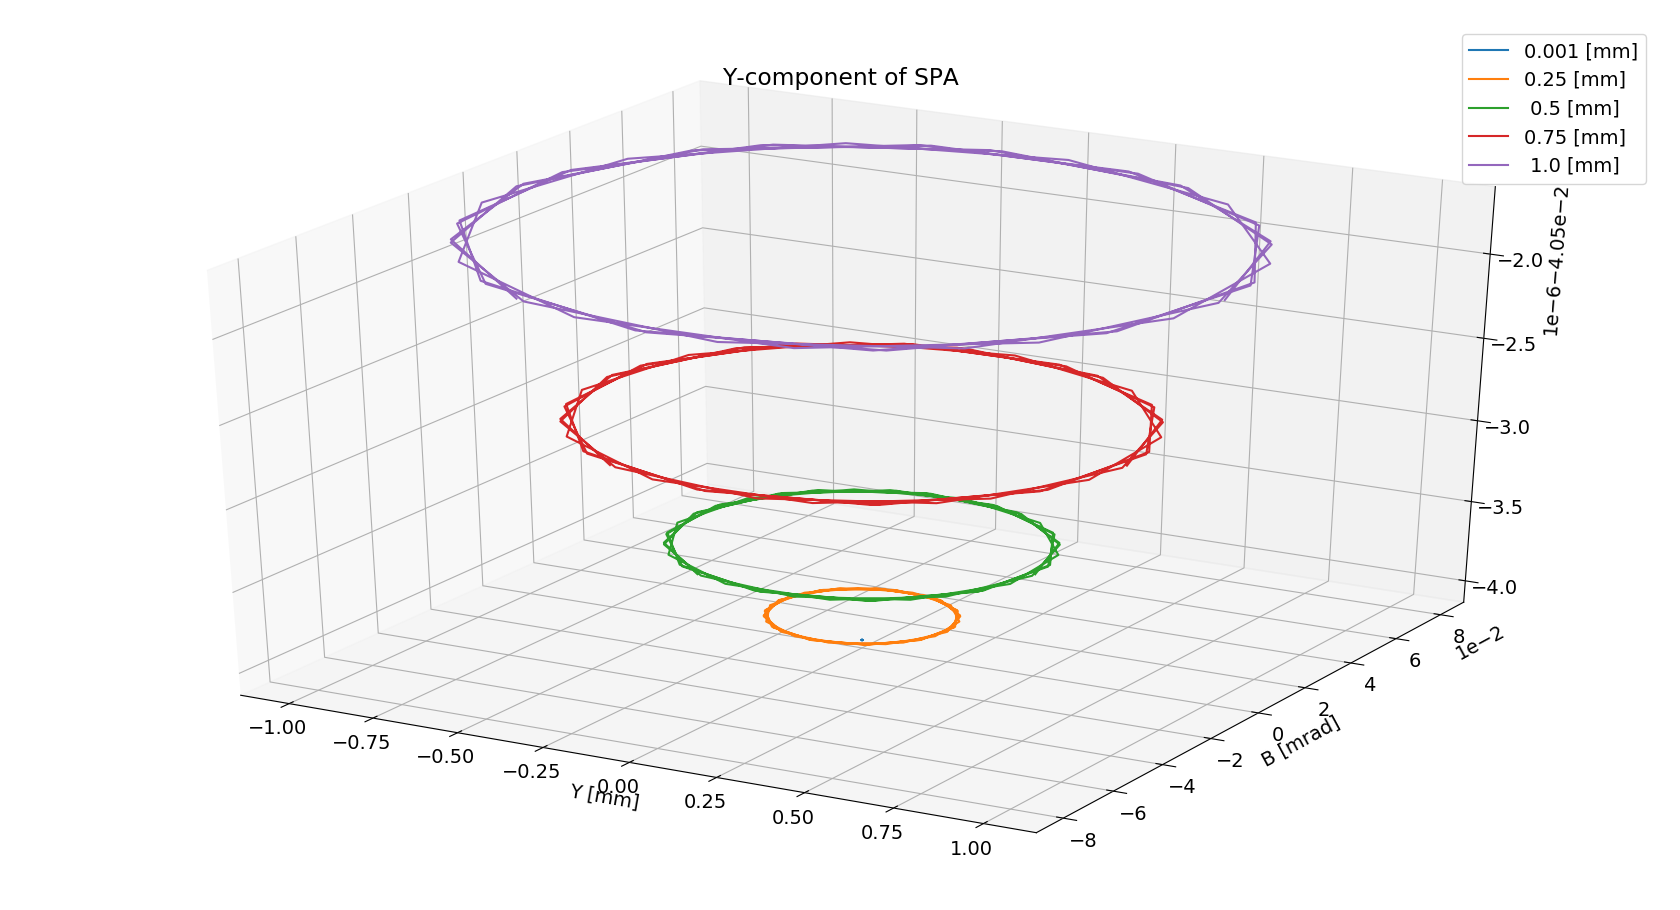
\includegraphics[width=\linewidth]{images/decoh_sim/NY_VS_YB_IMPERFECT_UNOPT}}
	\hfill
	\subbottom[С включенными секступолями.]{%
		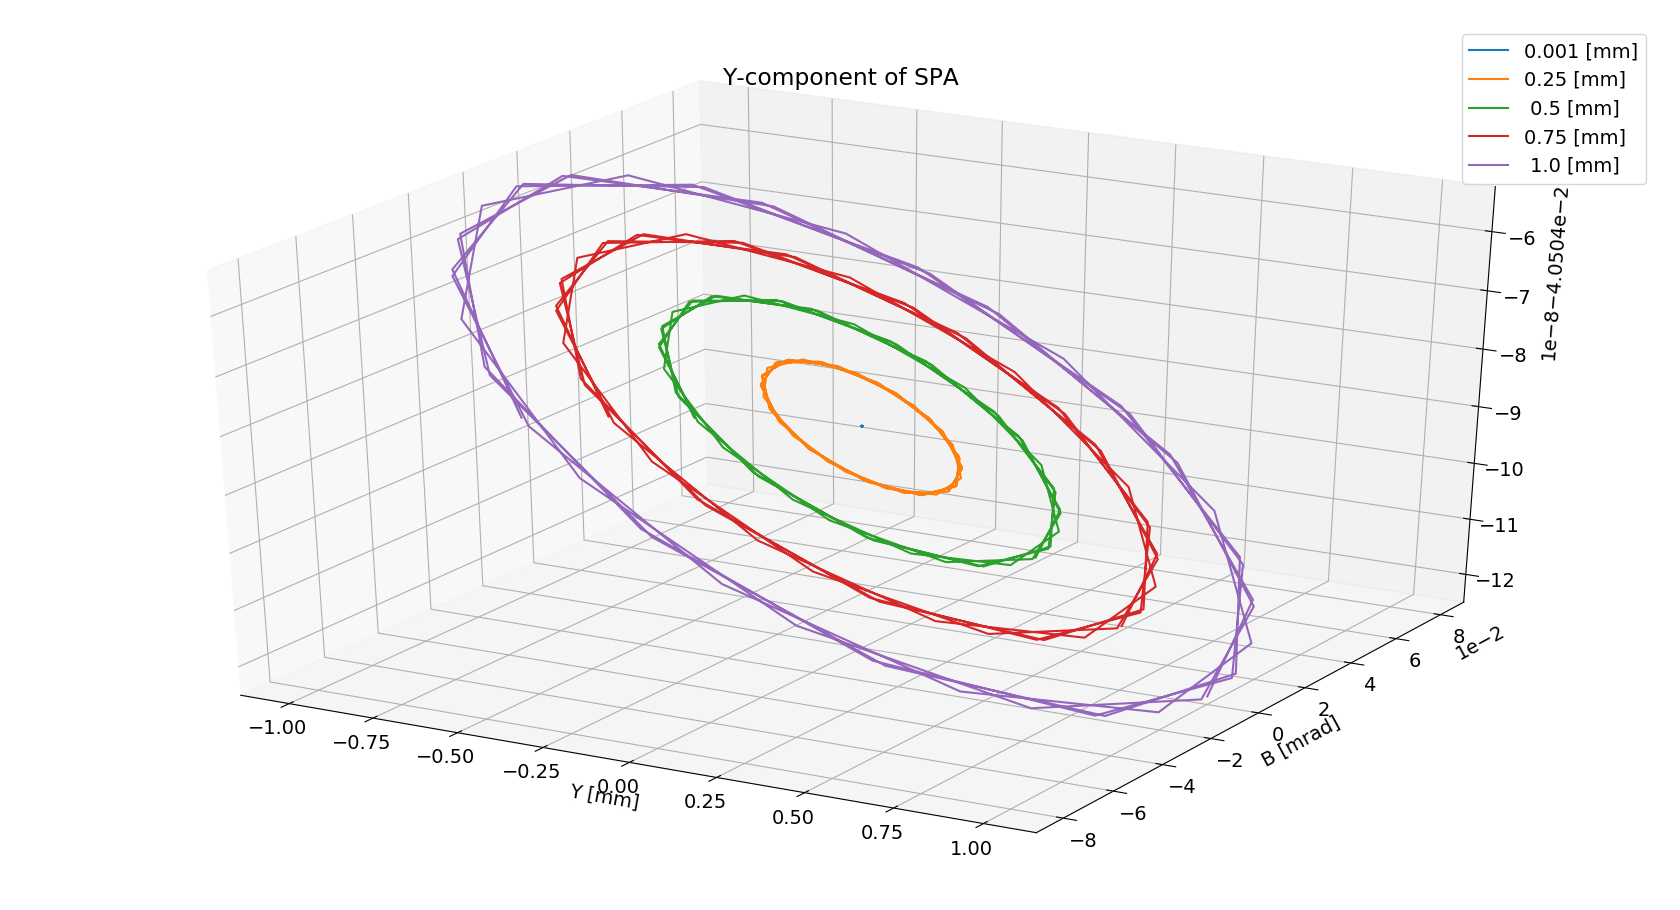
\includegraphics[width=\linewidth]{images/decoh_sim/NY_VS_YB_IMPERFECT_OPTIM}}
	\hfill
	\caption{Траектории и вертикальная компонента оси прецессии частиц в неидеальной FS-труктуре.\label{fig:ny_on_traj}}
\end{figure}

Исходя из рисунков можно отметить следующее:
\begin{enumerate}
	\item в безсекступольном случае, $\nu_s$ и направление $\bar n$ частицы в значительной мере фиксированы величиной её поперечного эмиттанса;
	\item при применении секступольных полей, уровни спин-тюна и компонент $\bar n$ частиц сравниваются, и становится виден эффект бетатронных колебаний, связанный с присутствием в разложении Тэйлора функций линейной компоненты.
\end{enumerate}

В частности, Рисунок~\ref{fig:ny_on_traj} свидетельствует о том, что применение секступольных полей не только выравнивает модули частот прецессии частиц банча, но и их направления.